\documentclass[10pt,a4paper]{article} 
\fontfamily{cmss}
\usepackage{amsmath}
\usepackage{amssymb}
\usepackage{mathtools}
\usepackage[brazilian]{babel}
\usepackage[utf8]{inputenc}
\usepackage[T1]{fontenc}
\usepackage[parfill]{parskip}
\usepackage[margin=1.0in]{geometry}
\usepackage{graphicx}
\usepackage{type1ec}
\usepackage{graphicx}
\usepackage{listings}
\usepackage[Algoritmo]{algorithm}
\usepackage[noend]{algpseudocode}
\usepackage{booktabs}

\begin{document}

	% CABECALHO %

	\begin{minipage}[b]{0.05\linewidth}
		%\begin{figure}
			
\includegraphics[scale=0.3]{ufmg}
		%\end{figure}
	\end{minipage}
	\hfill
	\begin{minipage}[b]{0.95\linewidth}
		\begin{flushright}
			\textbf{UNIVERSIDADE FEDERAL DE MINAS GERAIS} \\
			\textsc{Graduação em Engenharia de Sistemas} \\
			\textbf{Algoritmos e Estruturas de Dados III - Trabalho Prático 0} \\
			Operações de Nubby \\
			Matheus Silva Araujo - 2013066265
		\end{flushright}
	\end{minipage}

	\begin{center}
		\hrulefill
	\end{center}

	% CABECALHO %

	\section{Introdução}

	Este trabalho tem como objetivo comparar diferentes soluções para o problema \textit{Operações de Nubby}. O problema consiste na obtenção dos valores máximo, mínimo e soma em intervalos de um vetor de tamanho $n$.

	Os dois métodos a serem comparados são:

	\begin{itemize}

		\item \textbf{Matriz}: nesse método, será construída uma matriz $n \times n$ onde cada elemento $i \times j$ armazena os valores máximo, mínimo e soma do intervalo $i$ a $j$.
		\item \textbf{Árvore}: nesse método, será construída uma árvore de segmentação, onde cada nó de árvore representará os valores máximo, mínimo e soma de um determinado intervalo, e as folhas representam um intervalo de um elemento.

	\end{itemize}

	\section{Solução do Problema}

    Foram dados como entrada do problema: o vetor com os valores e também as operações nesse vetor:

    \begin{itemize}
        \item \textbf{Min} - Obter o menor valor em um intervalo $i \times j$
        \item \textbf{Max} - Obter o maior valor em um intervalo $i \times j$
        \item \textbf{Sum} - Obter a soma dos valores em um intervalo $i \times j$
        \item \textbf{Add} - Incrementar os valores em um intervalo $i \times j$
        \item \textbf{Sub} - Decrementar os valores em um intervalo $i \times j$
    \end{itemize}

    A saída deve ser o resultado das operações de consulta.

    Para as duas soluções foi utilizada uma estrutura do tipo $intervalo$, que contém os três valores inteiros: mínimo, máximo e soma. 

    A matriz é uma matriz dessa estrutura, e a árvore é armazenada em um vetor dessa estrutura.

    \subsection{Matriz}

    O método da matriz consiste em construir uma matriz simétrica $n \times n$, onde cada elemento $i \times j$ armazena os valores máximo, mínimo e soma do intervalo $i$ até $j$.

    O algoritmo para construir a matriz é bastante simples: dois laços percorrem o vetor de $1$ até $n$ com índices $i$ e $j$. A cada iteração os valores para o índice $i \times j$ são calculados com base nos valores do índice $i \times j-1$ e do elemento $j$ do vetor. O pseudo-código é mostrado no Algoritmo \ref{alg01}

    \begin{algorithm}[H]
    	\caption{Construção da Matriz.}
    	\label{alg01}

    	\begin{algorithmic}[1]
    		\For{i = 0 \textbf{to} n}
    			\State m[i,i].max $\gets$ v[i]
    			\State m[i,i].min $\gets$ v[i]
				\State m[i,i].sum $\gets$ v[i]
				\For{j = i + 1 \textbf{to} n}
					\State m[i,j].max $\gets$ m[j,i].max $\gets$ $max$(m[i,j-1].max, v[j])
					\State m[i,j].min $\gets$ ma[j,i].min $\gets$ $min$(m[i,j-1].min, v[j])
					\State m[i,j].sum $\gets$ ma[j,i].sum $\gets$ $sum$(m[i,j-1].sum, v[j])
				\EndFor
    		\EndFor
		\end{algorithmic}
        
    \end{algorithm}

    Para consultar os valores de um intervalo $i \times j$, basta acessar o elemento de índice $i \times j$.

    Nas operações de incremento e decremento, o vetor é atualizado e a matriz é reconstruída 
    \footnote{Seria possível implementar uma melhoria de forma que apenas o intervalo afetado pela alteração seja atualizado e não toda a matriz. No entanto, pelo anunciado do Trabalho Prático, essa poderia ser a solução. Pgs. 1 e 2}.

    \subsection{Árvore}

    O algoritmo de construção da árvore é uma função recursiva, onde se parte do intervalo $1$ a $n$ e a cada nova chamada o intervalo é partido ao meio até que se chegue a uma folha. Na folha, os valores de mínimo, máximo e soma são definidos como o valor correspondente do vetor. Para os demais nós, os valores são calculados em função dos valores dos filhos. O pseudo código é mostrado no algoritmo \ref{alg02}.

    \begin{algorithm}[H]
    	\caption{Construção da Árvore.}
    	\label{alg02}

		Entradas \\
		\textbf{ind} índice do nó atual no vetor da árvore \\
		\textbf{vi} índice inicial do intervalo \\
		\textbf{vf} índice final do intervalo \\

    	\begin{algorithmic}[1]
    		\If{vi = vf}
    			\State a[ind].min $\gets$ v[vi]
    			\State a[ind].max $\gets$ v[vi]
    			\State a[ind].sum $\gets$ v[vi]
    		\Else
    			\State vm $\gets$ valor médio entre vi e vf
    			\State e $\gets$ nó esquerdo, ind$*2+1$
    			\State d $\gets$ nó direito, ind$*2+2$

    			\State $construir$(vi, vm, e) \Comment{chamada recursiva}
    			\State $construir$(vm+1, vf, d) \Comment{chamada recursiva}

    			\State a[ind].min = $min$(a[e], a[d])
    			\State a[ind].max = $min$(a[e], a[d])
    			\State a[ind].sum = $sum$(a[e], a[d])
    		\EndIf
		\end{algorithmic}
        
    \end{algorithm}

    Um pseudo-código para a consulta na árvore é mostrado no algoritmo \ref{alg03}. O algoritmo para a atualização é semelhante, com a diferença de que em vez de consulta, ele faz uma atualização dos valores.

    \begin{algorithm}[H]
    	\caption{Consulta na Árvore.}
    	\label{alg03}

    	\begin{algorithmic}[1]
    		\If{o intervalo de consulta está totalmente \emph{dentro} do nó}
    			\State \textit{retornar valor solicitado}
    		\ElsIf{o intervalo de consulta está totalmente \emph{fora} do nó}
    			\State \textit{retonar elemento nulo}
			\Else
    			\State vm $\gets$ valor médio entre vi e vf
    			\State e $\gets$ nó esquerdo, ind$*2+1$
    			\State d $\gets$ nó direito, ind$*2+2$

    			\State $consultar$(vi, vm, e) \Comment{chamada recursiva}
    			\State $consultar$(vm+1, vf, d) \Comment{chamada recursiva}

				\State retornar função dos valores consutaltados nos nós
    		\EndIf
		\end{algorithmic}
        
    \end{algorithm}

	\section{Análise de Complexidade}

	Os dois algoritmos apresentam complexidades diferentes para a construção, atualização e consulta.

    \subsection{Matriz}

    \begin{itemize}
    	\item \textbf{Construção} A construção da matriz é um algortimo de ordem quadrática, pois necessita percorrer o vetor duas vezes para construí-la. Portanto $O(n^2)$.
    	\item \textbf{Atualização} A atualização da matriz é a mesma operação da Construção, $O(n^2)$.
    	\item \textbf{Consulta} A consulta na matriz é uma operação simples, bastando acessar uma posição. Portanto, $O(1)$.
    \end{itemize}

    \subsection{Árvore}

    \begin{itemize}
    	\item \textbf{Construção} A construção da árvore de segmentação tem custo $O(n)$. Há $2*n-1$ nós e o valor de cada nó é calculado apenas uma vez.
    	\item \textbf{Atualização} Para atualizar os nós, a complexidade é $O(log\, n)$. Ao atualizar uma folha, um nó em cada nível da árvore é atualizado.
    	\item \textbf{Consulta} A complexidade da consulta é a mesma da atualização $O(log\, n)$, pela mesma razão. Ao fazer uma consulta, no pior caso, todos os níveis da árvore serão visitados.
    \end{itemize}

    \section{Uso de memória}

    Os dois algoritmos também se diferem na utilização da memória.

    \subsection{Matriz}

    O algoritmo da matriz utiliza uma matriz $n \times n$, portano irá utilizar $n * n$ posições de memória.
    \footnote{Por ser uma matriz simétrica também, uma outra melhoria possível para o algoritmo seria armazenar apenas os elmentos $i \times j$ onde $i > j$.}

    \subsection{Árvore}

    No algoritmo da árvore de segmentação, a altura da árvore é $log_2 n$, e a memória utilizada será $2 * 2 log_2 n - 1$ posições de memória.

	\section{Avaliação Experimental}

	Para avaliar o desempenho das duas soluções foram feitos diversos testes onde o tamanho do vetor foi mantido fixo, $100$, e a quantidade de operações de consulta e atualização foram modificadas entre 0 e 100, os resultados são apresentados na Tabela \ref{tab01}. Um gráfico com esses resultados é apresentado na Figura \ref{fig01}.
    
	Os testes foram executados em uma máquina virtual com Linux Ubuntu. As medidas de tempo foram feitas pelo comando \textit{time}.

	\begin{table}[H]
		\centering
		\caption{Resultados das execuções}
		\label{tab01}
		\begin{tabular}{@{}llll@{}}
			\toprule 
			Alterações & Consultas & Matriz (s) & Árvore (s) \\ \midrule
			0 & 100 & 0.001  & 0.001 \\
			10 & 90 & 0.002 &  0.001 \\
			20 & 80 & 0.003 &  0.001 \\
			30 & 70 & 0.005 &  0.001 \\
			40 & 60 & 0.005 &  0.001 \\
			50 & 50 & 0.006 &  0.001 \\
			60 & 40 & 0.011 &  0.001 \\
			70 & 30 & 0.007 &  0.001 \\
			80 & 20 & 0.008 &  0.001 \\
			90 & 10 & 0.008 &  0.001 \\
			100 & 0 & 0.009 &  0.001 \\ \bottomrule
		\end{tabular}
	\end{table}

	\begin{figure}[H]
		\centering
		\caption{Resultados da execuções}
		\label{fig01}
		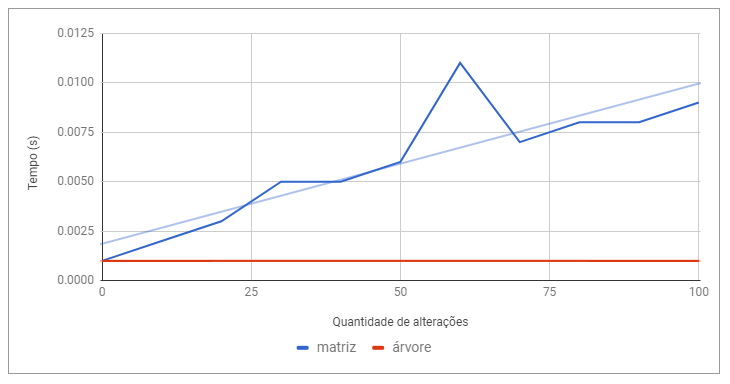
\includegraphics[scale=0.65]{tempos}
	\end{figure}

	\section{Conclusão}

	Como era imaginado pela análise de complexidade dos algoritmos, quando a quantidade de operações de alterações aumenta, o algoritmo de Matriz tem pior desempenho, enquanto o algoritmo da árvore de segmentação mantém o mesmo tempo de execução.

	Os dois algoritmos solucionam o mesmo problema com diferentes tempos para diferentes configurações das entradas. O algoritmo da árvore tem melhor desempenho no caso geral, no entanto sua implementação é mais complexa e as operações de consulta nele são mais lentas. Dessa forma, a escolha de um ou outro algoritmo irá depender das características do problema real que se deseja resolver.

\end{document}
